\documentclass[UTF8]{ctexart}
\usepackage{ctex}
\usepackage{geometry}
\usepackage{enumitem}
\usepackage{indentfirst}
\usepackage{color}
\usepackage{fancyhdr}
\usepackage{amsmath}
\usepackage{graphicx}
\usepackage{amssymb}
\usepackage{tikz}
\usepackage{cases}
\usepackage{array}
\usepackage{pgfplots}
\usepackage{tkz-euclide}
\usepackage{mathrsfs}
% 设置纸张和页边距——A4
\geometry{papersize={21cm,29.7cm}}
\geometry{left=3.18cm,right=3.18cm,top=2.54cm,bottom=2.54cm}

% 一级标题靠左
\CTEXsetup[format={\Large\bfseries}]{section}

% 去除页眉
\pagestyle{plain}

%设置段间距
\addtolength{\parskip}{.4em}
%%设置行间距
%\usepackage{setspace}
%\setstretch{2.5}

% 开始文档内容
\begin{document}

\title{信号与系统课程笔记:Lecture 30:系统的状态空间分析2}
\author{授课教师:秦雨潇 \\
        笔记记录:曹时成}
\date{2023 年 12 月 22 日(第十六周,周五)}
\maketitle

\section{课堂回顾}
\subsection{ }
\begin{figure}[h]
  \centering         %使图片居中放置
  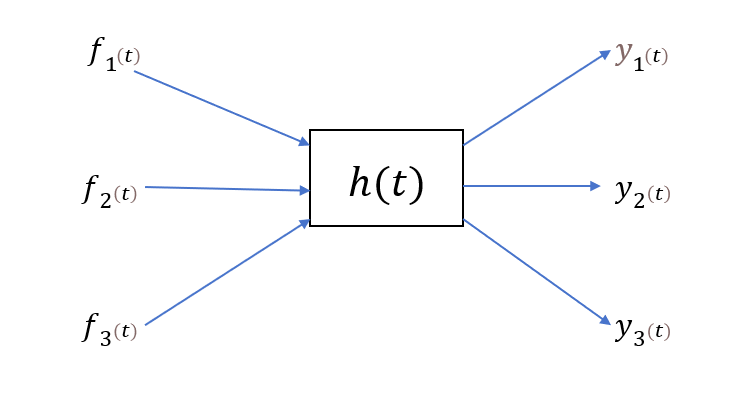
\includegraphics[scale=0.38]{1.png}
\end{figure}
(1)SISO   “Single Input Single output” \par
\qquad \quad $\Downarrow $ \par
\qquad MIMO   “Multiple Input Multiple output” \par
(2)h(t):黑盒子 \par
\qquad \quad $\Downarrow $ \par
\qquad 状态方程 \par

\subsection{例1:一个经典电路}
$\dot{X} = AX+ BF $ \quad “状态方程组 $\longrightarrow $ 矩阵形式” \par
(1)列方程 \par
\qquad  $[ x_1,x_2,\cdots ,x_n]^T$ \quad  必须一阶微分 \par
(2)解x \par
 (3)$Y=CX+DF$ \par

\section{例2:微分方程1}
$y'''(t)+ay''(t)+by'(t)+cy(t)=df(t)$  \par
解:3阶列3个  \par
\qquad $X=[x_1(t),x_2(t),x_3(t)]^T$  \par
(1)状态方程 \par
令:$x_1(t)=y(t),x_2(t)=y'(t),x_3(t)=y''(t)$  \par
则:\par
\qquad $x_1'=x_2(t)$  \par
\qquad $x_2'=x_3(t)$  \par
\qquad $x_3'=-ax_3(t)-bx_2(t)-cx_1(t)+df(t)$  \par
\begin{equation}
        \left[   
           \begin{matrix}
           x_1' \\
           x_2' \\
           x_3' \\
           \end{matrix}
         \right]
         =  \left[   
           \begin{matrix}
           0 &  1 & 0  \\
           0 &  0 & 1  \\
           -c & -b & -a  \\
           \end{matrix}
         \right]
         \left[   
          \begin{matrix}
          x_1 \\
          x_2 \\
          x_3 \\
          \end{matrix}
        \right]
        +\left[   
          \begin{matrix}
          0 \\
          0 \\
          d \\
          \end{matrix}
        \right]
        \left[   
          \begin{matrix}
          f_t \\
          \end{matrix}
        \right]
        \nonumber
       \end{equation}
\begin{equation}
        \dot{X} = AX+ BF
\nonumber
\end{equation}
(2)输出方程 \par
 $y=x_1$  \par
 \section{例3:微分方程2}
 $y'''(t)+ay''(t)+by'(t)+cy(t)=df(t)+ef'(t)+gf''(t)$  \par
 解: \par
 (1)状态方程 \par
换元: \par
\qquad $q'''(t)+aq''(t)+bq'(t)+cq(t)=f(t)$  \par
\qquad $y(t)=dq(t)+eq'(t)$  \par
\qquad $x_1'=x_2(t)$  \par
\qquad $x_2'=x_3(t)$  \par
\qquad $x_3'=-ax_3(t)-bx_2(t)-cx_1(t)+f(t)$  \par
(2)输出方程 \par
$y=dx_1+ex_2+gx_3$  \par
\section{例4:离散差分方程1}
$y[k]+ay[k-1]+by[k-2]=df[k]$  \par
解: \par
(1)状态方程 \par
原则:连续 “'”,放左边;离散“+1”,放左边 \par
$x_1[k]=y[k-2],x_2[k]=x_1[k+1],x_3[k]=x_2[k+1]$ \qquad 必须列成$x[k+1]$ 的形式!\par
$x_1[k+1]=x_2[k]$ \par
$x_2[k+1]=x_3[k]=-ax_1[k]-bx_2[k]+f[k]$ \par
$\dot{X} = AX+ BF$\par
(2)输出方程与例2中连续微分方程相同 \par
\section{例5:离散差分方程2}
同理于例3 \par
\section{9.3 解状态/输出方程}
\subsection{ }
$\dot{x} = Ax(t)+ Bf(t)$\par
对两边做laplace变换 \par
$ sX(s)-x(0^-)=AX(s)+BF(s) $ \par
$ (sI-A)X(s)=x(0^-)+BF(s) $ \par
$ X(s)=(sI-A)^{-1}(x(0^-)+BF(s)) $ \par
令:$ \Phi (s)=(sI-A)^{-1} $ \par
则:\par
\qquad $X(s)= \Phi (s)x(0^-)+\Phi (s)BF(s) $ \par
其中:\par
$\Phi (s)x(0^-)$ \qquad \qquad  为零输入响应 \par
$\Phi (s)BF(s) $ \qquad \qquad  为零状态响应 \par
$H(s)= \Phi (s)B $ \qquad \; 为系统函数 \par
$x(t)=\mathscr{L}^{-1}\{X(s)\}= \varphi (t)x(0^-)+\varphi (t)Bf(t) $  \par
输出方程:\par
$Y(s)=CX(s)+DF(s)$ \par
$Y(s)=C\Phi (s)x(0^-)+(C\Phi (s)B+D)F(s) $  \par
其中:\par
$C\Phi (s)x(0^-)$ \qquad \qquad  \quad 为零输入响应 \par
$(C\Phi (s)B+D)F(s) $ \qquad \, 为零状态响应 \par
$C\Phi (s)B+D=H(s) $ \qquad 为系统函数 \par
$y(t)=C\varphi (t)x(0^-)+(C\varphi (t)B+D)f(t) $  \par
\subsection{例题}
\begin{equation}
  \left[   
     \begin{matrix}
     x_1' \\
     x_2' \\
     \end{matrix}
   \right]
   =  \left[   
     \begin{matrix}
     -1 &  0   \\
     1 &  -3   \\
     \end{matrix}
   \right]
   \left[   
    \begin{matrix}
    x_1 \\
    x_2 \\
    \end{matrix}
  \right]
  +\left[   
    \begin{matrix}
    1 \\
    0 \\
    \end{matrix}
  \right] f_t
  \nonumber
 \end{equation}
 \begin{equation}
   y(t)=  \left[   
     \begin{matrix}
     -\frac{1}{2} &  1   \\
     \end{matrix}
   \right]
   \left[   
    \begin{matrix}
    x_1 \\
    x_2 \\
    \end{matrix}
  \right]
  +\left[   
    \begin{matrix}
    1 \\
    \end{matrix}
  \right] f_t ,f(t)=u(t),
  \left[   
    \begin{matrix}
    x_1(0^-) & x_2(0^-) \\
    \end{matrix}
  \right]^T=
  \left[   
    \begin{matrix}
    1 \\
    2 \\
    \end{matrix}
  \right]
  \nonumber
 \end{equation}
 解: \par
 (1) \par
\begin{equation}
  \Phi (s)=(sI-A)^{-1}=
  \left(
    \left[   
      \begin{matrix}
      s & 0 \\
      0 & s \\
      \end{matrix}
    \right]-
    \left[   
      \begin{matrix}
      -1 & 0 \\
      1 & -3 \\
      \end{matrix}
    \right]
  \right)^{-1}
= \left[   
  \begin{matrix}
  s-1 & 0 \\
  1 & s-3 \\
  \end{matrix}
 \right]^{-1}  
 \nonumber
\end{equation}
\begin{equation}
 = -\frac{1}{(s+3)(s+1)}
 \left[   
  \begin{matrix}
  s+3 & 0 \\
  1 & s+1 \\
  \end{matrix}
 \right]^{-1} 
 = \left[   
  \begin{matrix}
    \frac{1}{(s+1)} & 0 \\
    \frac{1/2}{(s+1)}-\frac{1/2}{(s+3)} & \frac{1}{(s+3)} \\
  \end{matrix}
 \right]
 \nonumber
\end{equation}
\quad (2)$\Phi (s) \longrightarrow \varphi (t)$ \par
\begin{equation}
  \varphi (t)= 
  \left[   
   \begin{matrix}
   e^{-t} & 0 \\
   \frac{1}{2}(e^{-t}-e^{-3t}) & e^{-3t} \\
   \end{matrix}
  \right]u(t) 
  \nonumber
 \end{equation}
 \quad (3)$C\Phi (s)B+D=H(s) $ \par
 \qquad \qquad \qquad \qquad $=\frac{1/2}{s+3}$ \par
(4) \par
 $y(t)=C\varphi (t)x(0^-)+\mathscr{L}^{-1}\{H(s)F(s)\} $  \par
\section{9.4 系统的稳定性判定}
$det(sI-A)=0$ \par
所有的根 s<0 时,则稳定

\end{document}